% ============================================================
\section{EV Power--Traffic Dynamic Coupling: CTM, Smart Charging, Dynamic OPF, and Carbon Flow}
\label{sec:ev_power_traffic_dynamic_model}
% ============================================================

This chapter replaces the earlier mixed description with a cleaner research
and implementation contract for the \texttt{hacdcpf::evpt} module. The
scientific model is a dynamic coupling of three infrastructures: traffic flow
is propagated by the cell transmission model (CTM), charging stations provide
flexible charging and V2G discharging, and the power network is operated by
repeated or embedded DC optimal power flow (DC-OPF). Renewable injections and
carbon-flow accounting are treated explicitly as the next layer needed for a
strong IEEE Transactions contribution.

The section separates three things that must not be conflated:
\begin{enumerate}
  \item the implemented C++ entry points and their numerical tests;
  \item the paper-level mathematical formulation that should be claimed;
  \item the literature-review and contribution evidence still needed from a
        Web of Science export.
\end{enumerate}

\begin{remark}[No hidden claim upgrade]
  The current source tree already implements CTM propagation, smart charging,
  V2G, CTM--DC-OPF price coordination, and a solver-certified LP/MILP joint
  optimizer. It does \emph{not} yet implement one monolithic CTM--smart
  charging--renewable dynamic-OPF--carbon-flow MILP. Where this chapter gives
  the full paper formulation, it is labelled as the target model. Where it
  reports tests, it reports only the source code that is currently present.
\end{remark}

% ------------------------------------------------------------
\subsection{Contribution Logic and Literature-Review Protocol}
\label{sec:evpt-literature-protocol}
% ------------------------------------------------------------

The contribution should be stated only after a reproducible literature screen.
The intended Web of Science search is not a cosmetic bibliography exercise: it
is the evidence used to decide whether the paper is mainly a traffic--power
co-optimization paper, or whether it needs the carbon-flow layer to become
sharp enough.

\begin{center}
\begin{tabularx}{\textwidth}{L{0.22\textwidth}X}
\toprule
\textbf{Question} & \textbf{Search intent} \\
\midrule
CTM and EV routing & Papers combining cell transmission or dynamic traffic
assignment with EV charging station choice. \\
Smart charging and V2G & Papers optimizing flexible charging/discharging after
traffic arrival, including station capacity and SOC limits. \\
Power-network operation & Papers coupling EV routing/charging with OPF,
especially dynamic or time-indexed OPF with renewable injections. \\
Carbon-aware coupling & Papers tracing carbon intensity through power flows and
using it in EV charging/routing decisions. \\
Infrastructure nature & Papers exposing how road bottlenecks, station limits,
renewable availability, and carbon intensity jointly reshape EV mobility. \\
\bottomrule
\end{tabularx}
\end{center}

The helper script \texttt{tools/wos\_evpt\_literature\_query.py} performs this
screen through the Clarivate Web of Science API when a key is available. In
this environment no \texttt{WOS\_API\_KEY},
\texttt{WEB\_OF\_SCIENCE\_API\_KEY}, or \texttt{CLARIVATE\_API\_KEY} variable
is present, so a live API query was not executed. The script therefore provides
the reproducible protocol rather than fabricated search results.

\paragraph{Working contribution hypothesis.}
Before the Web of Science export is available, the safest high-impact claim is:
\begin{quote}
  A dynamic EV mobility--charging--grid framework that preserves CTM traffic
  propagation, station-level flexible charging/V2G, and time-indexed power
  operation, and that can be extended with carbon-flow tracing to reveal how
  road, station, renewable, and carbon infrastructures jointly constrain EV
  travel.
\end{quote}
If the literature screen finds that CTM+smart-charging+OPF is already crowded,
the carbon-flow part should become a first-order contribution rather than a
minor post-processing metric.

% ------------------------------------------------------------
\subsection{Implemented Module Boundary}
\label{sec:evpt-module-structure}
% ------------------------------------------------------------

\begin{center}
\small
\begin{tabularx}{\textwidth}{L{0.23\textwidth}L{0.26\textwidth}X}
\toprule
\textbf{Entry point} & \textbf{Source file} & \textbf{Implemented role} \\
\midrule
\texttt{simulate\_ev\_power\_traffic()} &
\texttt{ev\_power\_traffic\_simulation.cpp} &
Route assignment, station-session synthesis, heuristic smart charging/V2G,
queue summaries, and optional ex-post power-flow validation. \\
\texttt{simulate\_ev\_power\_traffic\_ctm\_due()} &
\texttt{ctm\_propagation.cpp} &
Daganzo CTM forward propagation with route-specific commodities and MSA dynamic
user equilibrium. Charging sessions are synthesized after CTM convergence. \\
\texttt{simulate\_ev\_power\_traffic\_ctm\_joint()} &
\texttt{ctm\_joint\_welfare.cpp} &
Formulation C: CTM-DUE with repeated per-step DC-OPF and LMP-based station price
updates. \\
\texttt{solve\_joint\_social\_welfare()} &
\texttt{joint\_social\_welfare.cpp} &
Static assignment LP coupled to repeated DC-OPF price feedback; retained as a
baseline. \\
\texttt{solve\_joint\_optimizer()} &
\texttt{joint\_optimizer.cpp} &
Formulation D current code path: one solver-certified LP/MILP with free-flow
route columns, aggregate charging/V2G variables, station limits, and optional
embedded DC-OPF. \\
\texttt{compute\_carbon\_analysis()} &
\texttt{carbon\_analysis.cpp} &
Carbon-flow tracing exists in \texttt{hacdcpf::analysis}, but is not yet wired
into EVPT objectives or result types. \\
\bottomrule
\end{tabularx}
\end{center}

\begin{remark}[Dead-code and naming cleanup]
  New code should use \texttt{JointOptimizerMode::IntegerRouteMILP} for the
  integer route-flow variant. The old name
  \texttt{JointOptimizerMode::UserEquilibriumMILP} remains as a backward-
  compatible alias, but it does not assemble Wardrop complementarity. Likewise
  \texttt{AssignmentModel::SystemOptimal} is a legacy alias for the capacity-
  aware greedy model; exact assignment uses \texttt{SystemOptimalLP} or
  \texttt{SystemOptimalMILP}. These aliases are kept for compatibility rather
  than removed abruptly.
\end{remark}

% ------------------------------------------------------------
\subsection{Time Grid, Sets, and Data Contracts}
\label{sec:evpt-sets}
% ------------------------------------------------------------

The simulation grid is
\[
  \mathcal{T}=\{0,1,\ldots,K-1\},\qquad t_k=k\Delta t,
\]
where \(\Delta t\) is \texttt{EVPowerTrafficOptions::time\_step\_hr}. The CTM
uses a refined grid \(\mathcal{T}^{\mathrm{ctm}}\) with step
\(\Delta t_{\mathrm{ctm}}\). The power-network coupling uses the simulation
grid unless a future rolling-horizon dynamic OPF introduces a finer grid.

\begin{center}
\begin{tabular}{lll}
\toprule
\textbf{Symbol} & \textbf{Meaning} & \textbf{C++ data type} \\
\midrule
\(\mathcal{A}\) & directed traffic links & \texttt{TrafficLink} \\
\(\mathcal{R}\) & route alternatives & \texttt{RouteAlternative} \\
\(\mathcal{D}\) & EV travel demands & \texttt{EVDemand} \\
\(\mathcal{S}\) & charging stations & \texttt{ChargingStation} \\
\(\mathcal{B}\) & AC buses & \texttt{ACBus} \\
\(\mathcal{G}\) & controllable generators & \texttt{Generator} \\
\(\mathcal{L}\) & AC branches & \texttt{ACBranch} \\
\(\mathcal{Q}\) & renewable/static injections & \texttt{RenewableGen}, \texttt{PVSystem}, \texttt{StaticGenerator} \\
\bottomrule
\end{tabular}
\end{center}

% ------------------------------------------------------------
\subsection{CTM Traffic Flow Propagation}
\label{sec:evpt-traffic}
% ------------------------------------------------------------

The traffic layer should be described by CTM, not by static BPR delay, when the
paper claims dynamic road propagation. Each link \(a\in\mathcal{A}\) is split
into \(M_a\) cells of length \(\delta_a\). The CFL condition is
\begin{equation}
  \Delta t_{\mathrm{ctm}} \le \min_{a\in\mathcal{A}} \frac{\delta_a}{v^f_a},
  \label{eq:evpt-cfl}
\end{equation}
with free-flow speed \(v^f_a\). The implementation auto-selects
\(\Delta t_{\mathrm{ctm}}\) when \texttt{CTMOptions::dt\_ctm\_hr=0}.

Let \(n_{a,m,\kappa}\) be occupancy of cell \((a,m)\) at CTM step \(\kappa\),
and let \(q^{\max}_{a,\kappa}\) be the effective capacity after availability
and capacity profiles are applied. With backward wave speed \(w_a\) and jam
occupancy \(N^{\mathrm{jam}}_{a,m}\), CTM sending and receiving are
\begin{align}
  S_{a,m,\kappa}
  &= \Delta t_{\mathrm{ctm}}
     \min\!\left(\frac{v^f_a}{\delta_a}n_{a,m,\kappa},
                 q^{\max}_{a,\kappa}\right),
     \label{eq:evpt-send} \\
  R_{a,m,\kappa}
  &= \Delta t_{\mathrm{ctm}}
     \min\!\left(q^{\max}_{a,\kappa},
        \frac{w_a}{\delta_a}\left(N^{\mathrm{jam}}_{a,m}-n_{a,m,\kappa}\right)
     \right).
     \label{eq:evpt-recv}
\end{align}
The realized inter-cell flow is
\begin{equation}
  y_{a,m,\kappa}=\min(S_{a,m,\kappa},R_{a,m+1,\kappa}),
  \label{eq:evpt-intercell}
\end{equation}
and conservation is
\begin{equation}
  n_{a,m,\kappa+1}
  =n_{a,m,\kappa}+y_{a,m-1,\kappa}-y_{a,m,\kappa}.
  \label{eq:evpt-cell-update}
\end{equation}

At network nodes, incoming demand and outgoing supply are reconciled by a
proportional merge/diverge rule. For route-specific commodities \(r\), turning
fractions \(\phi^r_{a,b}\) preserve the station-choice identity:
\begin{equation}
  y^r_{a\rightarrow b,\kappa}
  = \phi^r_{a,b}\,\eta_{v,\kappa}\,S^r_{a,M_a,\kappa},
  \qquad 0\le \eta_{v,\kappa}\le 1.
  \label{eq:evpt-node-model}
\end{equation}
The CTM result reports station arrivals \(\lambda_{s,k}\), route travel times
\(T^{\mathrm{ctm}}_{r,k}\), and optional cell histories. These quantities are
validated in \texttt{test\_ev\_power\_traffic\_ctm\_due.cpp}.

\paragraph{Dynamic user equilibrium.}
The route-flow vector \(x\) is updated by method of successive averages:
\begin{equation}
  x^{(i+1)} = x^{(i)} + \alpha_i\left(\hat x^{(i)}-x^{(i)}\right),
  \qquad \alpha_i=1/i,
  \label{eq:evpt-msa}
\end{equation}
where \(\hat x^{(i)}\) is a deterministic shortest-path or logit assignment
under the current CTM experienced costs. The reported Wardrop relative gap is
\begin{equation}
  g^{\mathrm{DUE}}
  =\frac{\sum_{d,r}x_{d,r}C_{d,r}-\sum_d \bar d_d C^{\min}_d}
         {\max\left(\epsilon,\sum_d \bar d_d C^{\min}_d\right)}.
  \label{eq:evpt-ward-gap}
\end{equation}

% ------------------------------------------------------------
\subsection{Phase I: Multi-Class CTM-DUE with Heterogeneous Vehicles}
\label{sec:evpt-phase1-multiclass}
% ------------------------------------------------------------

Phase~I extends Formulation~B to a \emph{multi-class} dynamic user
equilibrium where internal-combustion vehicles (ICV) and electric vehicles
(EV) share road capacity. The two classes have different value-of-time,
fuel cost, and charging incentives, which leads to different route choices
even when travel times are identical. A passenger-car-equivalence (PCE)
weighting factor \(\gamma^c\) scales heterogeneous vehicle sizes onto a
common headway unit so that a single CTM forward pass governs congestion for
both classes simultaneously.

\subsubsection{Sets and Parameters}

Let \(\mathcal{C}=\{\mathrm{EV},\mathrm{ICV}\}\) be the set of vehicle
classes. The class-specific demand sets are
\(\mathcal{D}^{\mathrm{EV}}\) (\texttt{EVDemand}) and
\(\mathcal{D}^{\mathrm{ICV}}\) (\texttt{ICVDemand}).
Each class has a PCE factor \(\gamma^c>0\), a value-of-time
\(\mathrm{VOT}^c\) [\$/hr], and—for ICVs—a fuel cost \(\phi^{\mathrm{fuel}}_d\)
[\$/km]. For EVs, the cost of charging energy is captured through the station
price term carried from Formulation~B.

\subsubsection{PCE-Weighted CTM}

For each link \(a\), cell \(m\), and CTM step \(\kappa\), let
\(n^c_{a,m,\kappa}\) be the per-class cell occupancy (vehicles of
class \(c\)). The PCE-weighted combined occupancy is
\begin{equation}
  \tilde{n}_{a,m,\kappa}
  = \sum_{c\in\mathcal{C}} \gamma^c n^c_{a,m,\kappa}.
  \label{eq:evpt-pce-occ}
\end{equation}
The CTM sending and receiving functions
\eqref{eq:evpt-send}--\eqref{eq:evpt-recv} are evaluated on
\(\tilde{n}_{a,m,\kappa}\), yielding a combined inter-cell flow
\(\tilde{y}_{a,m,\kappa}=\min(\tilde{S}_{a,m,\kappa},\tilde{R}_{a,m+1,\kappa})\).
The per-class share of this flow is allocated proportionally:
\begin{equation}
  y^c_{a,m,\kappa}
  = \frac{\gamma^c n^c_{a,m,\kappa}}{\max\bigl(\varepsilon,\tilde{n}_{a,m,\kappa}\bigr)}
    \,\tilde{y}_{a,m,\kappa},
  \qquad c\in\mathcal{C}.
  \label{eq:evpt-per-class-flow}
\end{equation}
Class-specific cell updates then follow \eqref{eq:evpt-cell-update}
with \(y^c\) in place of \(y\). The combined route flow passed to the CTM is
\begin{equation}
  \tilde{x}_{r,k} = \gamma^{\mathrm{EV}}\, x^{\mathrm{EV}}_{r,k}
                  + \gamma^{\mathrm{ICV}}\, x^{\mathrm{ICV}}_{r,k}.
  \label{eq:evpt-combined-route-flow}
\end{equation}

\subsubsection{Per-Class Generalized Cost}

After a CTM forward pass, the experienced route travel time
\(T^{\mathrm{ctm}}_{r,k}\) is common to both classes (it is the
physical travel time on route \(r\) for departures at CTM step \(k\)).
The class-specific generalized costs are
\begin{align}
  c^{\mathrm{ICV}}_{r,k}
  &= T^{\mathrm{ctm}}_{r,k}
   + \frac{\phi^{\mathrm{fuel}}_d}{\mathrm{VOT}^{\mathrm{ICV}}}\,d_r,
  \label{eq:evpt-icv-cost} \\
  c^{\mathrm{EV}}_{r,k}
  &= T^{\mathrm{ctm}}_{r,k}
   + \frac{\omega_s\,\pi_{s(r),k}}{\mathrm{VOT}^{\mathrm{EV}}}\,e^{\mathrm{req}}_{r}
   + \Psi^{\mathrm{RA}},
  \label{eq:evpt-ev-cost}
\end{align}
where \(d_r\) is the total driving distance of route \(r\) [km],
\(\omega_s\) is the station energy cost weight, and
\(\Psi^{\mathrm{RA}}\) is the range-anxiety penalty.

\paragraph{Road failure.}
When link \(a\) is unavailable at CTM step \(\kappa\)
(\texttt{TrafficLink::available\_profile[}\(\kappa\)\texttt{] = false} or
\texttt{available = false}), the effective capacity is \(q^{\max}_{a,\kappa}=0\).
No vehicles are admitted to that link. The step-result reports
\(T_{a,\kappa}=+\infty\) so that the auxiliary assignment automatically excludes
all routes passing through the closed link. This is implemented by detecting
\(q^{\max}_{a,\kappa}=0\) in the per-link summary step and setting
\texttt{mean\_travel\_time\_hr = std::numeric\_limits<double>::infinity()}.

\subsubsection{Multi-Class MSA-DUE}

Each MSA iteration updates EV and ICV flows independently:
\begin{equation}
  x^{c,(i+1)}_{r,k}
  = \bigl(1-\alpha_i\bigr)\,x^{c,(i)}_{r,k}
  + \alpha_i\,\hat{x}^{c,(i)}_{r,k},
  \qquad \alpha_i=\frac{1}{i},\quad c\in\mathcal{C},
  \label{eq:evpt-multiclass-msa}
\end{equation}
where \(\hat{x}^{c,(i)}\) is the all-or-nothing assignment under the
current generalized cost \eqref{eq:evpt-icv-cost}--\eqref{eq:evpt-ev-cost}.
After the update, the combined route flow \(\tilde{x}\)
\eqref{eq:evpt-combined-route-flow} is recomputed for the next CTM pass.

Per-class Wardrop relative gaps are computed separately:
\begin{equation}
  g^c
  = \frac{\displaystyle\sum_{d\in\mathcal{D}^c,r}
    x^c_{d,r}\,c^c_{r,k_d}
    -\sum_{d\in\mathcal{D}^c}\bar d^c_d\,\hat{c}^c_{d,k_d}}
    {\displaystyle\max\!\left(\varepsilon,\,\sum_{d\in\mathcal{D}^c}\bar d^c_d\,\hat{c}^c_{d,k_d}\right)},
  \qquad c\in\mathcal{C}.
  \label{eq:evpt-perclass-gap}
\end{equation}
The overall stopping criterion is \(g=\max_{c\in\mathcal{C}}g^c<\epsilon\).
Convergence requires that each class is at its own Wardrop equilibrium,
not merely the combined flow.

\subsubsection{C++ Implementation}

The multi-class logic is activated by \texttt{CTMOptions::enable\_multiclass
= true} and the PCE fields \texttt{ev\_pce}, \texttt{icv\_pce}. The
problem carries \texttt{std::vector<ICVDemand> icv\_demands} alongside the
existing \texttt{std::vector<EVDemand> demands}. Inside
\texttt{simulate\_ev\_power\_traffic\_ctm\_due()}, two parallel
\(T_{\mathrm{ctm}}\times R\) arrays \texttt{x\_ev} and \texttt{x\_icv}
are maintained; the combined PCE route flow is assembled before each CTM
forward pass. The result types \texttt{CTMDUEResult::PerClassStats} and
\texttt{CTMDUEResult::flow\_by\_icv\_route} carry the per-class
outputs. The EV-class Wardrop gap is correctly computed on \texttt{x\_ev}
(not on the combined \texttt{route\_flow}) to avoid an inflated TSTT term
from ICV vehicles.

\subsubsection{Phase~I Test Cases}

\begin{center}
\small
\begin{tabularx}{\textwidth}{L{0.08\textwidth}L{0.20\textwidth}X}
\toprule
\textbf{ID} & \textbf{Name} & \textbf{Verified property} \\
\midrule
P1-1 & EV baseline &
  With \texttt{enable\_multiclass=false} and no \texttt{icv\_demands},
  the result is identical to Formulation~B (class\_stats empty,
  total flow = demand, DUE converged). \\
P1-2 & Mixed ICV+EV &
  4~EVs + 6~ICVs on a 2-route network; per-class stats populated,
  total ICV flow = 6, total EV flow = 4, DUE converges. \\
P1-3 & Cell-state tracking &
  High EV demand on a low-capacity route with
  \texttt{record\_cell\_history=true}; cell history is non-empty
  and total inflow to links is positive. \\
P1-4 & Road failure and rerouting &
  Route-1 links set \texttt{available=false}; both EVs and ICVs are
  routed entirely to route~2 because unavailable links report
  \(T^{\mathrm{ctm}}_{r,k}=+\infty\). \\
P1-5 & Differential class routing &
  EVs prefer route~1 (low electricity price); ICVs also prefer the
  shorter route; class\_stats has two entries with correct totals
  and non-negative TSTT values. \\
\bottomrule
\end{tabularx}
\end{center}

% ------------------------------------------------------------
\subsection{Station Smart Charging and V2G}
\label{sec:evpt-sessions}
% ------------------------------------------------------------

For a charging session \(v\) arriving at station \(s(v)\), the flexible
variables are charging power \(p^{ch}_{v,k}\), discharge power
\(p^{dis}_{v,k}\), and stored energy \(e_{v,k}\). The generic smart-charging
subproblem is
\begin{align}
  \min \quad
  &\sum_{v,k}\pi_{s(v),k}\left(p^{ch}_{v,k}-p^{dis}_{v,k}\right)\Delta t
    + M_E\sum_v \ell^E_v,
    \label{eq:evpt-smart-obj} \\
  e_{v,k+1}
  &=e_{v,k}+\eta^{ch}_v p^{ch}_{v,k}\Delta t
      -\frac{p^{dis}_{v,k}\Delta t}{\eta^{dis}_v},
    \label{eq:evpt-smart-energy} \\
  \underline e_v A_{v,k}
  &\le e_{v,k}\le \overline e_v A_{v,k},
    \label{eq:evpt-smart-soc} \\
  0&\le p^{ch}_{v,k}\le \overline p^{ch}_v A_{v,k},
    \label{eq:evpt-smart-ub-ch} \\
  0&\le p^{dis}_{v,k}\le \overline p^{dis}_v A_{v,k},
    \label{eq:evpt-smart-ub-dis} \\
  e_{v,k^{dep}_v}+\ell^E_v&\ge e^{tar}_v.
    \label{eq:evpt-smart-slack}
\end{align}
The station limits are
\begin{align}
  \sum_{v:s(v)=s} p^{ch}_{v,k} &\le \overline P^{ch}_{s,k},
    \label{eq:evpt-station-charge} \\
  \sum_{v:s(v)=s} p^{dis}_{v,k} &\le \overline P^{dis}_{s,k}.
    \label{eq:evpt-station-discharge}
\end{align}
The C++ code uses two implementations of this idea: a greedy price-threshold
dispatcher in \texttt{ev\_power\_traffic\_simulation.cpp} and
\texttt{ctm\_propagation.cpp}, and an exact aggregate LP/MILP version inside
\texttt{joint\_optimizer.cpp}. The exact version can add binary mode variables
\(\delta^{ch}_{v,k}\), \(\delta^{dis}_{v,k}\) so that
\begin{equation}
  p^{ch}_{v,k}\le \overline p^{ch}_v\delta^{ch}_{v,k},\qquad
  p^{dis}_{v,k}\le \overline p^{dis}_v\delta^{dis}_{v,k},\qquad
  \delta^{ch}_{v,k}+\delta^{dis}_{v,k}\le 1.
  \label{eq:evpt-charge-discharge-mode}
\end{equation}

% ------------------------------------------------------------
\subsection{Dynamic OPF and Renewable Operation}
\label{sec:evpt-power-coupling}
% ------------------------------------------------------------

The power-system layer is time-indexed. In Formulation C, each simulation step
solves a DC-OPF after injecting the CTM-derived EV station load. In the current
Formulation-D LP/MILP, DC-OPF variables are embedded directly in the same model
as the route and charging variables.

For bus \(b\), branch \(\ell=(i,j)\), and step \(k\), a dynamic DC-OPF target
with renewable treatment is
\begin{align}
  \sum_{g\in\mathcal{G}_b} P^g_{g,k}
  + P^{ren}_{b,k}-P^{curt}_{b,k}
  - P^d_{b,k}-P^{EV}_{b,k}
  - \sum_{\ell:i=b} f_{\ell,k}
  + \sum_{\ell:j=b} f_{\ell,k}
  &=0,
  \label{eq:evpt-dopf-balance} \\
  f_{\ell,k} &= B_{\ell}\left(\theta_{i,k}-\theta_{j,k}\right),
  \label{eq:evpt-dopf-flow} \\
  -\overline f_{\ell} &\le f_{\ell,k}\le \overline f_{\ell},
  \label{eq:evpt-dopf-branch} \\
  0\le P^g_{g,k}&\le \overline P^g_g,
  \qquad 0\le P^{curt}_{b,k}\le P^{ren}_{b,k}.
  \label{eq:evpt-dopf-renew}
\end{align}
The operating objective is
\begin{equation}
  C^{grid}=\sum_{k,g} c_g P^g_{g,k}\Delta t
  +\sum_{k,b} c^{curt}_{b,k}P^{curt}_{b,k}\Delta t
  +\sum_{k,b} M^p \ell^p_{b,k}.
  \label{eq:evpt-dopf-obj}
\end{equation}

\begin{remark}[Current renewable status]
  The standalone \texttt{solve\_dc\_opf()} path already accounts for
  \texttt{StaticGenerator}, \texttt{RenewableGen}, and \texttt{PVSystem} as
  fixed injections in the bus balance. The EVPT Formulation-C loop inherits
  that behavior because it calls \texttt{solve\_dc\_opf()} at every step. The
  embedded Formulation-D LP currently includes controllable \texttt{Generator}
  dispatch only; explicit renewable curtailment variables \(P^{curt}\),
  renewable forecasts, storage intertemporal constraints, and AC-OPF/MINLP
  variants remain target-model work.
\end{remark}

The LMP update used in Formulation C is
\begin{equation}
  \pi^{(i+1)}_{s,k}
  = \alpha\frac{\lambda^{(i)}_{b(s),k}}{1000}
    +(1-\alpha)\pi^{(i)}_{s,k},
  \label{eq:evpt-price-update}
\end{equation}
where \(\lambda\) is in \$/MWh and station prices are in \$/kWh.

% ------------------------------------------------------------
\subsection{Carbon-Flow Extension}
\label{sec:evpt-carbon-flow}
% ------------------------------------------------------------

If the literature screen shows that CTM+smart-charging+OPF is not sufficiently
distinctive, the strongest available extension is carbon-flow-aware EV
operation. The repository already includes proportional tracing and a
matrix-based carbon-intensity solve in \texttt{src/carbon\_analysis}. For each
time step, after EV loads are injected and a power-flow or OPF result is
available, the carbon-analysis module can compute bus carbon intensity
\(\chi_{b,k}\) [tCO2/MWh].

The station carbon price seen by EVs is then
\begin{equation}
  c^{CO2}_{s,k}=\rho^{CO2}_{k}\,\chi_{b(s),k}/1000,
  \label{eq:evpt-carbon-price}
\end{equation}
where \(\rho^{CO2}_k\) is a carbon price [\$/tCO2]. The smart-charging
objective becomes
\begin{equation}
  \sum_{v,k}\left(\pi_{s(v),k}+c^{CO2}_{s(v),k}\right)
       \left(p^{ch}_{v,k}-p^{dis}_{v,k}\right)\Delta t.
  \label{eq:evpt-carbon-aware-charge}
\end{equation}
This makes the infrastructure contribution sharper: two stations with the same
electricity LMP can have different carbon consequences because their upstream
generation mix and losses differ.

% ------------------------------------------------------------
\subsection{Integrated Formulations}
\label{sec:evpt-formulations}
% ------------------------------------------------------------

\subsubsection{Formulation B: CTM-DUE}
\label{sec:evpt-ctm-due}

Formulation B is the implemented dynamic traffic model:
\[
  \text{route flows}\;x
  \longrightarrow
  \text{CTM propagation}\;(n,y,T^{ctm},\lambda)
  \longrightarrow
  \text{MSA route update}.
\]
It is the correct place to claim road spillback, queue propagation, and
experienced dynamic travel time. It is \emph{not} a power-system optimizer.
Charging sessions and station loads are synthesized after CTM-DUE convergence.

\subsubsection{Formulation C: CTM-DUE with Dynamic DC-OPF}
\label{sec:evpt-ctm-joint}

Formulation C is the implemented infrastructure coordination loop:
\begin{algorithm}[H]
\caption{CTM-DUE and dynamic DC-OPF price coordination}
\begin{algorithmic}[1]
\State Initialize station prices \(\pi^{(0)}_{s,k}\)
\For{outer iteration \(i=1,2,\ldots\)}
  \State Run CTM-DUE with prices \(\pi^{(i-1)}\)
  \State Dispatch smart charging/V2G for CTM-derived sessions
  \For{each step \(k\)}
    \State Inject station EV load into the power network
    \State Solve DC-OPF and extract LMPs \(\lambda_{b,k}\)
    \State Update \(\pi_{s,k}\) by Eq.~\eqref{eq:evpt-price-update}
  \EndFor
  \State Stop if the maximum price change is below tolerance
\EndFor
\end{algorithmic}
\end{algorithm}
This is a fixed-point coordination method. It has CTM propagation and
time-indexed OPF, but it is not one monolithic optimization certificate.

\subsubsection{Formulation D: Current Solver-Certified LP/MILP}
\label{sec:evpt-formulation-d}

The implemented Formulation-D path is the exact LP/MILP currently assembled by
\texttt{joint\_optimizer.cpp}. Its route timing is free-flow, not CTM. Its
traffic constraint is route-capacity screening, not cell propagation. Its EV
charging and V2G variables are aggregate session variables, not per-vehicle
plug assignment. Within those boundaries it is solver-certified.

The main variables are route flow \(h_{d,r}\), unserved demand \(u_d\),
aggregate session power \(p^{ch},p^{dis}\), battery energy \(e\), optional
mode binaries, and optional DC-OPF variables \((P^g,\theta,f,\ell^p)\). The
current social-welfare minimization objective is
\begin{equation}
  \min\;\sum_{g,k}c_g P^g_{g,k}\Delta t
      -\sum_{d,r} B_d h_{d,r}
      +\sum_{d,r} \mathrm{VOT}\,T^{ff}_{r}h_{d,r}
      +\sum_d M^{trip}u_d
      +\sum_{b,k}M^p\ell^p_{b,k}.
  \label{eq:evpt-d-social-objective}
\end{equation}
The user-benefit minimization objective is
\begin{equation}
  \min\;\sum_{v,k}\pi_{s(v),k}\left(p^{ch}_{v,k}-p^{dis}_{v,k}\right)\Delta t
      -\sum_{d,r} B_dh_{d,r}
      +\sum_{d,r}\mathrm{VOT}\,T^{ff}_{r}h_{d,r}
      +\sum_d\left(M^{trip}+\Omega_d\right)u_d.
  \label{eq:evpt-d-user-objective}
\end{equation}
Electricity appears only through \(p^{ch}-p^{dis}\); it is not duplicated on
route-flow columns.

\paragraph{Target D-CTM extension.}
The paper-level integrated model should replace free-flow route timing by CTM
constraints \eqref{eq:evpt-send}--\eqref{eq:evpt-node-model}, keep the
smart-charging constraints
\eqref{eq:evpt-smart-energy}--\eqref{eq:evpt-station-discharge}, and couple
them to dynamic OPF constraints
\eqref{eq:evpt-dopf-balance}--\eqref{eq:evpt-dopf-renew}. This gives a true
dynamic infrastructure model, but it is not yet the current
\texttt{solve\_joint\_optimizer()} implementation.

% ------------------------------------------------------------
\subsection{Numerical Verification and Publication Figures}
\label{sec:evpt-numerical-verification}
% ------------------------------------------------------------

\begin{center}
\small
\begin{tabularx}{\textwidth}{L{0.13\textwidth}X L{0.16\textwidth}}
\toprule
\textbf{Test group} & \textbf{Verified behavior} & \textbf{Status} \\
\midrule
Formulation A & Static route assignment, station capacities, unserved demand,
system-optimal LP/MILP, and reporting. & pass \\
Formulation B & CTM propagation, route-specific commodities, MSA-DUE,
SOC feasibility, and price-of-anarchy diagnostics. & pass \\
Phase~I (multi-class) & Multi-class CTM-DUE with ICV+EV demand, PCE-weighted
capacity sharing, per-class Wardrop gaps, road failure\,/\,rerouting
(\(T=+\infty\) for closed links), and cell-history recording
(P1-1 through P1-5). & pass \\
Formulation C & CTM-DUE plus repeated DC-OPF price coordination and welfare
history. & pass \\
Formulation D & Single LP/MILP route--charging--V2G--DC-OPF subset,
objective accounting, road availability rows, outside-option cost, and MIP
certificate fields. & pass \\
\bottomrule
\end{tabularx}
\end{center}

The latest full test run discovered 481 CTest entries: 479 passed and 2
MATPOWER cases were skipped by design. Case Study D has 10 tests and 94
assertions.

\begin{figure}[H]
\centering
\begin{tikzpicture}[
  node distance=9mm and 10mm,
  block/.style={rectangle,rounded corners=2pt,draw=blue!55!black,fill=blue!5,
                align=center,text width=3.0cm,minimum height=9mm},
  target/.style={rectangle,rounded corners=2pt,draw=teal!65!black,fill=teal!8,
                 align=center,text width=3.35cm,minimum height=9mm},
  line/.style={-Latex,thick}
]
\node[block] (ctm) {CTM traffic\\propagation};
\node[block,right=of ctm] (charge) {station smart\\charging and V2G};
\node[block,right=of charge] (opf) {dynamic DC-OPF\\with renewables};
\node[target,below=of charge] (carbon) {carbon-flow tracing\\fallback contribution};
\draw[line] (ctm) -- node[above,align=center]{\scriptsize arrivals,\\[-1mm]\scriptsize travel times} (charge);
\draw[line] (charge) -- node[above,align=center]{\scriptsize EV load,\\[-1mm]\scriptsize V2G injection} (opf);
\draw[line] (opf) -- (carbon);
\draw[line] (carbon) -- node[left]{\scriptsize carbon price} (charge);
\end{tikzpicture}
\caption{Infrastructure-centered paper narrative. The contribution should be
verified as a dynamic interaction among road propagation, station flexibility,
power-network operation, and carbon intensity, not merely as a route-choice
example.}
\label{fig:evpt-infrastructure-narrative}
\end{figure}

\begin{figure}[H]
\centering
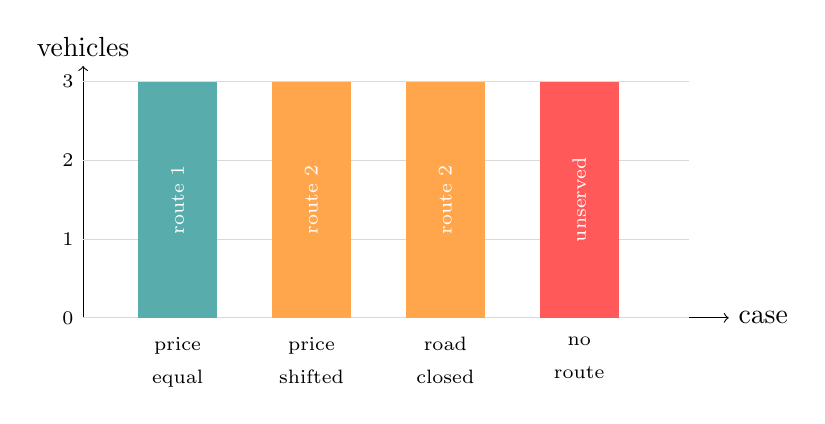
\begin{tikzpicture}[x=1cm,y=1cm]
\draw[->] (0,0) -- (8.2,0) node[right]{case};
\draw[->] (0,0) -- (0,3.2) node[above]{vehicles};
\foreach \y/\lab in {0/0,1/1,2/2,3/3} {
  \draw[black!15] (0,\y) -- (7.7,\y);
  \node[left] at (0,\y) {\scriptsize \lab};
}
\fill[teal!65] (0.7,0) rectangle (1.7,3.0);
\fill[orange!70] (2.4,0) rectangle (3.4,3.0);
\fill[orange!70] (4.1,0) rectangle (5.1,3.0);
\fill[red!65] (5.8,0) rectangle (6.8,3.0);
\node[below,align=center] at (1.2,-0.12) {\scriptsize price\\\scriptsize equal};
\node[below,align=center] at (2.9,-0.12) {\scriptsize price\\\scriptsize shifted};
\node[below,align=center] at (4.6,-0.12) {\scriptsize road\\\scriptsize closed};
\node[below,align=center] at (6.3,-0.12) {\scriptsize no\\\scriptsize route};
\node[white,rotate=90] at (1.2,1.5) {\scriptsize route 1};
\node[white,rotate=90] at (2.9,1.5) {\scriptsize route 2};
\node[white,rotate=90] at (4.6,1.5) {\scriptsize route 2};
\node[white,rotate=90] at (6.3,1.5) {\scriptsize unserved};
\end{tikzpicture}
\caption{Certified infrastructure response in the current Formulation-D test
case: prices move charging-route choice, road availability removes a path, and
complete entry closure activates unserved-demand slack.}
\label{fig:evpt-d-infrastructure-response}
\end{figure}

% ------------------------------------------------------------
\subsection{Implementation Roadmap}
\label{sec:evpt-roadmap}
% ------------------------------------------------------------

\begin{description}
  \item[D1.] Keep the current LP/MILP optimizer as the certified baseline for
  route, aggregate charging/V2G, station limits, and optional embedded DC-OPF.
  \item[D2.] Add a CTM-constrained integrated model or a decomposition method
  whose master variables are route flows and station EV load, and whose traffic
  subproblem is CTM propagation.
  \item[D3.] Promote renewable operation from fixed OPF injections to explicit
  time-indexed renewable availability and curtailment variables.
  \item[D4.] Wire \texttt{compute\_carbon\_analysis()} into EVPT outputs and add
  carbon-aware station prices or objective terms.
  \item[D5.] Retire misleading legacy names gradually: prefer
  \texttt{IntegerRouteMILP}, \texttt{SystemOptimalLP}, and
  \texttt{SystemOptimalMILP}; keep old aliases only for compatibility.
  \item[D6.] Run the Web of Science script, export the screened records, and
  rewrite the contribution paragraph from evidence rather than intuition.
\end{description}

The final IEEE-style claim should be made only after D2--D4 are either
implemented or clearly presented as a future extension. At the present state,
the strongest honest paper framing is a validated software framework with a
solver-certified LP/MILP core, an implemented CTM--OPF coordination loop, and a
clear carbon-flow path for turning infrastructure operation into an emissions
contribution.